\chapter{Optimisation and Learning}
\section{Logistic Regression}
\subsection{Maximum Likelihood Predictor}
Maximum likelihood estimation is a method to estimate the parameters of a statistical model, which in the context of logistic regression, leads to finding the best coefficients for the predictors.\\

\textbf{1. Statistical Model Setup:}
\begin{itemize}
    \item We have a binary class \( y \) representing two possible outcomes, with \( y = +1 \) and for the event's occurrence and \(y=-1\) for it not occurring.
    \item Distribution \( P(y) \) for the class variable \( y \).
    \item Observations \( x_1, x_2, \ldots, x_d \) are independent binary features 0 or 1 that contribute to the prediction of $y$.
    \item Note that $x \in \{0,1\}$ and $y \in \{-1,1\}$
\end{itemize}

\textbf{2. Assumptions:}
\begin{itemize}
    \item We assume each feature $x_i$ is independent, and so:
    \[ P(x_1, \ldots, x_d|y) = P(x_1|y) \times \ldots \times P(x_d|y) \]
\end{itemize}

\textbf{3. Posterior Probability:}
\begin{itemize}
    \item With Bayes' rule, we have:
    \[ P(y|x_1, \ldots, x_d) = \frac{P(y) \times P(x_1, \ldots, x_d|y)}{P(x_1, \ldots, x_d)} \]
    \item Assuming feature independence:
    \[ P(y|x_1, \ldots, x_d) = \frac{P(y) \times \prod_{i=1}^{d} P(x_i|y)}{P(x_1, \ldots, x_d)} \]
\end{itemize}

\textbf{4. Odds and Log Odds:}
\begin{itemize}
    \item The odds of $y$ being 1 or -1 is the ratio of their respective probabilities. By independence, this the product of every feature's probability given y:
    \begin{align*}\frac{P(y=1|x_1,\ldots,x_d)}{P(y=-1|x_1,\ldots,x_d)}&=\frac{P(x_1|y=1)}{P(x_1|y=-1)}\times\ldots\times\frac{P(x_d|y=1)}{P(x_d|y=-1)}\times\frac{P(y=1)}{P(y=-1)}\end{align*}

    Taking the log of the odds make everything more mathematically convenient, and we see this starts to look like a linear model:
    \begin{align*}
    \log\frac{P(y=1|x_1,\ldots,x_d)}{P(y=-1|x_1,\ldots,x_d)}&=\log\frac{P(y=1)}{P(y=-1)}+\sum_{i=1}^{d}\log\frac{P(x_i|y=1)}{P(x_i|y=-1)}\\
&=w_0+ \sum_{i=1}^dw_i^*\mathbf{x}_i=\mathbf{w}_*^\top\mathbf{x}
    \end{align*}

As part of the training/learning process, we want to consider $P(x_i|y)$, which is the probability of our observations of the data, given a label $y$.
Since $x$ can only take on two values, we can specify $P(x_i|y)$ as a piecewise function:
\[
P(x_i|y)=
\begin{cases}
    P(x_i = 1 | y) & \text{if } x_i = 1 \\
P(x_i = 0 | y) & \text{if } x_i = 0
\end{cases} \]

When we take the logarithm of \( P(x_i | y) \), we are just applying the logarithm function to the above piecewise definition. However, we want a single equation that works for both cases (when \( x_i = 1 \) and \( x_i = 0 \)). To achieve this, we use \( x_i \) itself as a coefficient that becomes 1 when \( x_i = 1 \) and 0 when \( x_i = 0 \), and similarly, \( (1 - x_i) \) becomes 0 when \( x_i = 1 \) and 1 when \( x_i = 0 \).
Now, let's derive the equation:
For \( x_i = 1 \), the log probability is:
\[ \log P(x_i | y) = \log P(x_i = 1 | y) \]
For \( x_i = 0 \), the log probability is:
\[ \log P(x_i | y) = \log P(x_i = 0 | y) \]
Since \( x_i \) can only be 0 or 1, we can write the log probability as a single expression that accounts for both cases by using \( x_i \) and \( 1 - x_i \) as weights:
\[ \log P(x_i | y) = x_i \log P(x_i = 1 | y) + (1 - x_i) \log P(x_i = 0 | y) \]
What this does is select the correct log probability term based on the value of \( x_i \), `turning on' the first case and `turning off' the second case when $x_i = 1$, and vice versa when $x_i = 0$.

Expanding further, we get:
\begin{align*}
\log P(x_{i}|y)& =x_i\log P(x_i=1|y)+(1-x_i)\log P(x_i=0|y)  \\
&=x_{i}\bigg(\underbrace{\log P(x_{i}=1|y)-\log P(x_{i}=0|y)}_{\beta_{i,y} \text{ that depends on observation } x_i \in \{0,1\} \text{from the data}}\bigg)+\underbrace{\log P(x_{i}=0|y)}_{\gamma_{i,y} \text{ always added regardless of observation $x_i$}}\\
&= x_i(\beta_{i,y}) + \gamma_{i,y} \\
\text{where }& \beta_{i,y} = \log P(x_{i}=1|y)-\log P(x_{i}=0|y)\\
& \gamma_{i,y}=\log P(x_{i}=0|y)
\end{align*}

We use $\beta_{i,y}, \gamma_{i,y}$ to refer to parameters that are estimated from our data. \\

Going back to our log likelihood estimator and plugging in our values:

\begin{align*}
\log{\frac{P(x_{i}|y=1)}{P(x_{i}|y=-1)}}& =\log P(x_i|y=1)-\log P(x_i|y=-1)  \\
&= (x_i(\beta_{i,y=1}) + \gamma_{i, y=1}) - (x_i(\beta_{i,y=-1}) + \gamma_{i, y=-1})\\
&=x_{i}(\underbrace{\beta_{i,1}-\beta_{i,-1}}_{w_{i}^{*}})+\underbrace{(\gamma_{i,1}-\gamma_{i,-1})}_{w_0^*}
\end{align*}

We see this is very similar to a linear prediction model.
\end{itemize}

\textbf{5. Logistic Regression Model:}
\begin{itemize}
    \item Maximising the likelihood of the observed data through log-likelihood.
    \item We also relax binary and independence assumptions on $x_i$, so we can use numbers as more descriptive data features.\\

    With x=$(1,x_1,\ldots,x_d)$ and $y\in(-1,+1\}$, assume: 
    \begin{align*}&\log\frac{P(y=+1|x_1,\ldots,x_d)}{P(y=-1|x_1,\ldots,x_d)}=\mathbf{w}_*^\top\mathbf{x}=h(\mathbf{x},\mathbf{w})\end{align*}
    Using $P(y=-1|\mathbf{x})=P(y=-1|x_1,\ldots,x_d)=1-P(y=+1|x_1,\ldots,x_d)$, we have
    
    \begin{align*}
P(y=+1|\mathbf{x})&=\theta(\mathbf{w}_*^\top\mathbf{x})\\
    P(y=-1|\mathbf{x})&=1-\theta(\mathbf{w}_*^\top\mathbf{x})
    \end{align*}

    We get our logistic function
    \[P(y=1|\mathbf{x})=\frac{e^{\mathbf{w}_*^\top\mathbf{x}}}{1+e^{\mathbf{w}_*^\top\mathbf{x}}}=\frac1{1+e^{-\mathbf{w}_*^\top\mathbf{x}}}=\theta(\mathbf{w}_*^\top\mathbf{x})\]
    
We use $\mathbf{w}_*$ to refer to the set of weights that minimises the empirical error, the true and most accurate weight.
    
\end{itemize}
\begin{figure}[H]
    \centering
    \includegraphics[width=0.75\linewidth]{img/sigmoid.png}
    \caption{Sigmoid function}
    \label{fig:sigmoid-label}
\end{figure}
\subsection{Model Probabilities}
The probability of the outcome \( y \) given a predictor \( \mathbf{x} \) is modeled as:

\[
P(y|\mathbf{x}) = 
\begin{cases}
\theta(\mathbf{w}^\top\mathbf{x}) & \text{if } y = +1;\\
1 - \theta(\mathbf{w}^\top\mathbf{x}) & \text{if } y = -1,
\end{cases}
\]

where:
\begin{itemize}
    \item \( \theta(s) \) is the logistic function defined as \( \theta(s) = \frac{1}{1 + e^{-s}} \).
    \item \( \mathbf{w} \) is the weight vector.
    \item \( \mathbf{w}^\top\mathbf{x} \) is the dot product of the weight vector and the feature vector.
\end{itemize}

\subsubsection*{Likelihood Function}
The likelihood of an observed dataset \( D = \{(\mathbf{x}_1, y_1), \ldots, (\mathbf{x}_n, y_n)\} \) under the logistic regression model is given by the product of individual probabilities:

\[
L(\mathbf{w}) = \prod_{i=1}^{n} P(y_i|\mathbf{x}_i) = \prod_{i=1}^{n} \theta(y_i\mathbf{w}^\top\mathbf{x}_i).
\]

\subsubsection*{Log-Likelihood}
The log-likelihood, which transforms the product into a sum, making it computationally more convenient, is:

\[
\log L(\mathbf{w}) = \sum_{i=1}^{n} \log \theta(y_i\mathbf{w}^\top\mathbf{x}_i).
\]

To facilitate gradient-based optimisation, we minimise the negative of the log-likelihood:

\[
-\log L(\mathbf{w}) = -\sum_{i=1}^{n} \log \theta(y_i\mathbf{w}^\top\mathbf{x}_i) = \sum_{i=1}^{n} \log \left(1 + e^{-y_i\mathbf{w}^\top\mathbf{x}_i}\right).
\]

\subsection{Cross-Entropy Error}
The negative log-likelihood is equivalent to the cross-entropy error, which is commonly used as the error measure in logistic regression:

\[
\hat{R}_n(\mathbf{w}) = \frac{1}{n} \sum_{i=1}^{n} \log \left(1 + e^{-y_i\mathbf{w}^\top\mathbf{x}_i}\right).
\]

This cross-entropy error function is convex, and its minimisation leads to the maximum likelihood estimation of the model parameters \( \mathbf{w} \).

In logistic regression, the predicted probability for a positive class is modelled by the logistic function \( h(\mathbf{x}) \), defined as:
\[ h(\mathbf{x}) = \sigma(\mathbf{w}^\top \mathbf{x}) = \frac{1}{1 + e^{-\mathbf{w}^\top \mathbf{x}}} \]
The loss function, derived from the negative log-likelihood for the Bernoulli distribution, is given by:
\[ \ell(h(\mathbf{x}), y) = \begin{cases}
\log \frac{1}{h(\mathbf{x})} & \text{if } y = +1;\\
\log \frac{1}{1 - h(\mathbf{x})} & \text{if } y = -1.
\end{cases} \]
The cross-entropy error over a dataset is the average loss:
\[ \hat{R}_n = \frac{1}{n} \sum_{i=1}^{n} \left[ \mathbb{I}(y_i = +1) \log \frac{1}{h(\mathbf{x}_i)} + \mathbb{I}(y_i = -1) \log \frac{1}{1 - h(\mathbf{x}_i)} \right] \] where $\mathbb{I}$ is the indicator function that returns 1 when its argument evaluates to true, and -1 when false.
Considering entropy and cross-entropy:
\begin{itemize}
\item Entropy \( H(p) \) is:
\[ H(p) = p \log \frac{1}{p} + (1 - p) \log \frac{1}{1 - p} \]
\item Cross-entropy \( H(p, q) \) between two distributions \( p \) and \( q \) is:
\[ H(p, q) = p \log \frac{1}{q} + (1 - p) \log \frac{1}{1 - q} \]
\end{itemize}
Minimizing the cross-entropy error function during training optimises the weight vector \( \mathbf{w} \) to improve the predictive accuracy of the logistic regression model.


\subsection{Empirical Risk Minimisation for Logistic Regression}

The formula for empirical risk from linear regression is \[
\widehat R_n(\mathbf{w})=\frac1n\sum_{i=1}^n(y_i-\mathbf{w}^\top\mathbf{x}_i)^2
\] 

this is a convex problem that has a closed-form solution.\\

For logistic regression, however, we have 
\[
\widehat R_n(\mathbf{w})=\frac1n\sum_{i=1}^n\log\left(1+e^{-y_i\mathbf{w}^\top\mathbf{x}_i}\right);
\]

Which has no closed form solution. We require gradient descent.

\section{Gradient Descent}

Gradient descent is a widely-used optimization algorithm in machine learning, specifically for training logistic regression models. It iteratively adjusts model parameters to minimize the cost function, typically the cross-entropy loss.

\subsection{Direction of Descent}
The parameter update rule in gradient descent is given by:
\[ \mathbf{w}_{t+1} = \mathbf{w}_t + \eta\mathbf{v}, \]
where \( \mathbf{v} \) is the direction vector of the steepest descent, and \( \eta \) represents the learning rate.

\subsection{Step Size in Gradient Descent}
The learning rate \( \eta \) is crucial for the convergence of gradient descent:
\begin{itemize}
    \item A small \( \eta \) may slow down convergence.
    \item An overly large \( \eta \) can cause divergence.
    \item An adaptive \( \eta \) can improve convergence speed and stability.
\end{itemize}



\begin{sidenotebox}{More information on gradient descent}
If $\mathbf{v}=-\frac{\nabla\hat{R}_{n}(\mathbf{w}_{t})}{\|\nabla\hat{R}_{n}(\mathbf{w}_{t})\|}$, direction is defined by:
\begin{align*}\Delta\hat{R}_{n}&=\hat{R}_{n}(\mathbf{w}_{t+1})-\hat{R}_{n}(\mathbf{w}_{t})\\
&=\hat{R}_{n}(\mathbf{w}_{t}+\eta\mathbf{v})-\hat{R}_{n}(\mathbf{w}_{t})\\
&=\eta\nabla\hat{R}_{n}(\mathbf{w}_{t})^{\top}\mathbf{v}+O(\eta^{2})\geqslant-\eta\|\nabla\hat{R}_{n}(\mathbf{w}_{t})\|+O(\eta^{2})\end{align*}

The direction of the parameter update in gradient descent is key to effectively minimising the risk function \( \hat{R}_n \). The change in \( \hat{R}_n \) after an update is defined as:

\[ \Delta \hat{R}_n = \hat{R}_n(\mathbf{w}_{t+1}) - \hat{R}_n(\mathbf{w}_t) \]

Given the update rule \( \mathbf{w}_{t+1} = \mathbf{w}_t + \eta\mathbf{v} \), where \( \mathbf{v} \) is a unit vector and \( \eta \) is the learning rate, we can approximate the change in \( \hat{R}_n \) using a Taylor expansion:

\[ \hat{R}_n(\mathbf{w}_{t+1}) \approx \hat{R}_n(\mathbf{w}_t) + \eta \nabla \hat{R}_n(\mathbf{w}_t)^\top \mathbf{v} + O(\eta^2) \]

The optimal direction \( \mathbf{v} \) for the steepest descent is in the direction of the negative gradient, normalised:

\[ \mathbf{v} = -\frac{\nabla \hat{R}_n(\mathbf{w}_t)}{\| \nabla \hat{R}_n(\mathbf{w}_t) \|} \]

Incorporating this into the update rule, we achieve the gradient descent step:

\[ \mathbf{w}_{t+1} = \mathbf{w}_t - \eta \frac{\nabla \hat{R}_n(\mathbf{w}_t)}{\| \nabla \hat{R}_n(\mathbf{w}_t) \|} \]

This step ensures that the parameters are updated in the direction that most rapidly decreases the risk function \( \hat{R}_n \), taking into account the magnitude of the learning rate \( \eta \).
\end{sidenotebox}



\subsection{Empirical Risk Minimisation (ERM)}
In the context of logistic regression, ERM aims to find the optimal parameter vector \( \mathbf{w}^* \) by minimising the empirical risk \( \hat{R}_n(\mathbf{w}) \), the average loss over the dataset.


\begin{definitionbox}{Gradient Descent Algorithm}
\begin{itemize}
    \item Initialise the weight vector \( \mathbf{w}_0 \).
    \item For each iteration \( t \):
    \begin{enumerate}
        \item Compute the gradient of \( \hat{R}_n \) or \( \mathcal{L}_n \):
        \[ \nabla\hat{R}_n(\mathbf{w}_t) = -\frac{1}{n} \sum_{i=1}^{n} \frac{y_i\mathbf{x}_i}{1 + e^{y_i\mathbf{w}_t^\top\mathbf{x}_i}}. \]
        \item Update the weights:
        \[ \mathbf{w}_{t+1} = \mathbf{w}_t - \eta\nabla\hat{R}_n(\mathbf{w}_t). \]
        \item Repeat until a stopping condition is met.
    \end{enumerate}
    \item Return the final weights \( \mathbf{w}^* = \mathbf{w}_t \).
\end{itemize}    
\end{definitionbox}

\section{Stochastic Gradient Descent}
Each loss function \( \ell \) is utilised in empirical risk minimisation (ERM) for different regression and classification tasks:

\begin{itemize}
  \item Linear regression: \( \hat{R}_n(\mathbf{w}) = \frac{1}{n}\sum_{i=1}^n (y_i - \mathbf{w}^\top\mathbf{x}_i)^2 \)
  \item Logistic regression: \( \hat{R}_n(\mathbf{w}) = \frac{1}{n}\sum_{i=1}^n \log(1 + e^{-y_i\mathbf{w}^\top\mathbf{x}_i}) \)
  \item Classification: \( R_n(\mathbf{w}) = \frac{1}{n}\sum_{i=1}^n I(y_i \neq \text{sign}(\mathbf{w}^\top\mathbf{x}_i)) \) 
\end{itemize}

The loss function must be differentiable for gradient-based optimisation techniques. The general error for a hypothesis \( h \) is \( \hat{R}_n(h) = \frac{1}{n} \sum_{i=1}^n \ell(h(\mathbf{x}_i), y_i) \).\\

However, some measures of empirical risk include potential for non-convexity and computational issues, especially for high-dimensional data. However, using stochastic gradient descent, we can solve some of these issues through approximation.

\subsection*{Empirical Risk Minimisation with SGD}

Computing the full gradient $\widehat{R}_{n}(\mathbf{w})=\frac{1}{n}\sum_{i=1}^{n}\ell(\mathbf{w}_{t},\mathbf{x}_{i},y_{i})$ can be expensive, so stochastic Gradient Descent can approximate the minimisation of \( \hat{R}_n \) as follows:

\begin{commentbox}{Use of Notation}
    The slide notes refer to $\hat{R}_{n,t,i}$ as $\ell_{t,i}$ at a given iteration $n$.
\end{commentbox}

\begin{definitionbox}{Stochastic Gradient Descent Algorithm}
    \begin{itemize}
  \item Initialise \( \mathbf{w}_0 \).
  \item For \( i=1,2\ldots n \text{ and } t = 0,1,2,\ldots \)
  \begin{enumerate}
    \item Compute the gradient at a random point $(\mathbf{x}_i, y_i)$:
    \( \nabla\hat{R}_{n,t,i} = \frac{\partial \ell(\mathbf{w}_t, \mathbf{x}_i, y_i)}{\partial \mathbf{w}} \). Choose $i$ uniformly at random from $\{1,\ldots, n\}$
    \item Update the weights:
    \( \mathbf{w}_{t+1} = \mathbf{w}_t - \eta \nabla\hat{R}_{n,t,i} \)
    \item Repeat until a stopping criterion is met. This could be when the change in weights is minimum, validation error, etc.
  \end{enumerate}
  \item Return final weight \( \mathbf{w}^* = \mathbf{w}_t \).
\end{itemize}

Stochastic Gradient Descent (SGD) introduces a randomised element. In SGD, one sample $(\mathbf{x}_i, y_i)$ is selected at random for each iteration, and gradient descent is applied to the in-sample error for that specific point. The expected value of the stochastic gradient is equivalent to the full gradient:
\[ \mathbb{E}_i[\nabla\hat{R}_{n,t,i}] = \nabla\hat{R}_n(\mathbf{w}_t) \]

\end{definitionbox}
The efficacy of SGD comes from the expected (average) direction of the error gradient, which we aim to minimise. Mathematically, this is represented as:\\

\begin{align*}
\mathbb{E}_i\left[\nabla\hat{R}_{n,t,i}\right] &= \frac{1}{n}\sum_{n=1}^{n} \frac{\partial\ell(\mathbf{w}_{t},\mathbf{x}_{i},y_{i})}{\partial\mathbf{w}_{t}} \\
&= \nabla\hat{R}_n(\mathbf{w}_t)
\end{align*}

Intuitively, SGD is more computationally efficient as it operates on smaller samples, making calculations easier and quicker. Despite being a noisy approximation of the gradient over the entire dataset (as we are taking a small sample), this noise tends to average out over multiple iterations. Additionally, the randomised nature of SGD helps in avoiding local minima or maxima that are not globally optimal.\\

\subsection*{Hinge Loss}

\begin{commentbox}{Wrong Location???}
    The slides somehow place a definition here, but we will only utilise this in the next chapter on SVMs.
\end{commentbox}
The hinge loss is a loss function used primarily with Support Vector Machines (SVMs). It is defined as:
\begin{equation}
    \ell(w, x_i, y_i) = \max(0, 1 - y_i \langle w, x_i \rangle),
\end{equation}
where \( w \) is the weight vector, \( x_i \) is the input vector, and \( y_i \) is the true label of \( x_i \). The hinge loss penalizes predictions that are on the wrong side of the decision boundary, defined by a margin.

\subsection*{Gradient of Hinge Loss}
The gradient of the hinge loss, used to update the weights \( w \), is:
\begin{equation}
    \frac{\partial \ell}{\partial w} =
    \begin{cases}
        -y_i x_i & \text{if } y_i \langle w, x_i \rangle < 1, \\
        0 & \text{otherwise}.
    \end{cases}
\end{equation}
This gradient contributes to the update only when the predicted margin is incorrect or within the margin threshold.

\subsection*{Attributes of SGD with Hinge Loss}
SGD with hinge loss is characterized by the following attributes:
\begin{itemize}
    \item Efficiency, due to its stochastic nature and use of individual examples for gradient computation.
    \item Variants like minibatch SGD, which use a subset of the data at each iteration for a more stable gradient estimate.
    \item Flexibility, with different step sizes for different coordinates and non-uniform sampling strategies.
    \item Scalability, allowing distributed computation over large datasets.
\end{itemize}

\subsection*{Applications}
Hinge loss is predominantly used in training SVMs, aiming for a model that maximises the margin between different classes, enhancing the model's generalisation capabilities.

\subsubsection*{Rule of Thumb for Learning Rate:}
A common starting point for the learning rate $\eta$ is $0.1$, though it may require adjustment based on specific problem characteristics or dataset properties.

\section{Neural Networks}

The perceptron is just the model of a single neuron. We can combine them together to produce more complex hypothesis classes. Below we can implement logic gates and combinations of different hypotheses.

\begin{figure}[H]
    \centering
    \includegraphics[width=0.5\linewidth]{img/XORMLP.png}
    \caption{The XOR gate, unlike OR and AND requires two layers to be implemented as a Multilayer Perceptron.}
\end{figure}

Multilayer Perceptrons are poweful because they can implement non-linear classification boundaries:
\begin{figure}
    \centering
    \includegraphics[width=0.5\linewidth]{img/MLP-circle.png}
    
    
\end{figure}

% \subsection{Stochastic Gradient Descent}

% We have previously discussed standard gradient descent, also known as 'batch' gradient descent. In this approach, the objective is to minimise the in-sample error $E_{\mathrm{in}}(\mathbf{w})$, which is defined as:

% \[
% E_{\mathrm{in}}(\mathbf{w}) = \frac{1}{N}\sum_{n=1}^{N} \mathbf{e}\left(h(\mathbf{x}_{n}), y_{n}\right) = \frac{1}{N}\sum_{n=1}^{N} \ln\left(1 + e^{-y_{n}\mathbf{w}^{\mathrm{T}}\mathbf{x}_{n}}\right)
% \]

% In batch gradient descent, the hypothesis is evaluated at every point $n$ in the sample to determine the direction of the next iterative step, given by $\Delta \mathbf{w} = -\eta \nabla E_{\mathrm{in}}(\mathbf{w})$. This process involves computing the gradient based on all examples $(\mathbf{x}_n, y_n)$.\\

% In contrast, Stochastic Gradient Descent (SGD) introduces a randomised element. In SGD, one sample $(\mathbf{x}_n, y_n)$ is selected at random for each iteration, and gradient descent is applied to the in-sample error for that specific point, $\mathbf{e}\left(h(\mathbf{x}_{n}), y_{n}\right)$.\\





\begin{figure}[H]
    \centering
\begin{tikzpicture}
    % Define the style for the plots
    \pgfplotsset{
        myplot/.style={
            axis lines=middle,
            width=5cm,
            height=5cm,
            xlabel={$x_1$},
            ylabel={$x_2$},
            xtick=\empty,
            ytick=\empty,
            xmin=0, xmax=3,
            ymin=0, ymax=3,
            enlargelimits=false
        }
    }

    % Leftmost plot with the 'X'
    \begin{axis}[myplot]
        \addplot [no marks, domain=0.5:2.5, samples=2, thick] ({x},{0.5*x+0.5});
        \addplot [no marks, domain=0.5:2.5, samples=2, thick] ({x},{-0.5*x+2.5});
        \node at (axis cs:2.5,1.5) {$+$};
        \node at (axis cs:0.75,1.25) {$+$};
        \node at (axis cs:1.75,0.75) {$-$};
        \node at (axis cs:2 ,2.25) {$-$};
    \end{axis}

    % Middle plot with line h1
    \begin{axis}[myplot, at={(6cm,0)}]
        \addplot [no marks, domain=0.5:2.5, samples=2, thick] ({x},{0.5*x+0.5});
        \node at (axis cs:1.5,2) {$+$};
        \node at (axis cs:1.75,0.4) {$-$};
        \node[label={270:{$h_1$}}] at (axis cs:1.5,1.25) {};
    \end{axis}

    % Rightmost plot with line h2
    \begin{axis}[myplot, at={(12cm,0)}]
        \addplot [no marks, domain=0.5:2.5, samples=2, thick] ({x},{-0.5*x+2.5});
        \node at (axis cs:2,2.5) {$+$};
        \node at (axis cs:1,1.25) {$-$};
        \node[label={270:{$h_2$}}] at (axis cs:1.5,1.75) {};
    \end{axis}
\end{tikzpicture}
    \caption{Combining several perceptrons together helps us achieve classifications a single perceptron cannot achieve on its own.}
    \label{fig:multi-percep}
\end{figure}


\begin{figure}[H]
    \centering
\begin{tikzpicture}[>=Stealth, node distance=1.5cm]

    % OR Perceptron
    \node[input neuron] (input1) {$1$};
    \node[input neuron, below of=input1] (inputx1) {$x_1$};
    \node[input neuron, below of=inputx1] (inputx2) {$x_2$};

    \node[activation function, right of=inputx1] (activation1) {};
    % Draw step function inside the activation node for OR
    % \draw (activation1.south west) -- (activation1.south west -| activation1.west) -- (activation1.north west -| activation1.east) -- (activation1.north east);

    \node[output neuron, right=0.75cm of activation1] (output1) {};
    \draw[->] (activation1) -- (output1);

    \node[right=0.1cm of output1] (or) {OR$(x_1, x_2)$};

    \draw[->] (input1) -- (activation1) node[midway,above] {1.5};
    \draw[->] (inputx1) -- (activation1) node[midway,above] {1};
    \draw[->] (inputx2) -- (activation1) node[midway,above] {1};

    % AND Perceptron
    \node[input neuron, right=6cm of input1] (input3) {$1$};
    \node[input neuron, below of=input3] (inputx3) {$x_1$};
    \node[input neuron, below of=inputx3] (inputx4) {$x_2$};

    \node[activation function, right of=inputx3] (activation2) {};
    % Draw step function inside the activation node for AND
    % \draw (activation2.south west) -- (activation2.south west -| activation2.west) -- (activation2.north west -| activation2.east) -- (activation2.north east);

    \node[output neuron, right=0.75cm of activation2] (output2) {};
    \draw[->] (activation2) -- (output2);

    \node[right=0.1cm of output2] (and) {AND$(x_1, x_2)$};

    \draw[->] (input3) -- (activation2) node[midway,above] {-1.5};
    \draw[->] (inputx3) -- (activation2) node[midway,above] {1};
    \draw[->] (inputx4) -- (activation2) node[midway,above] {1};

\end{tikzpicture}
    \caption{Implementing AND and OR gates with perceptrons}
    \label{fig:multi-percep2}
\end{figure}


\subsection{How a neural network operates}
\begin{figure}[H]
    \centering
    \includegraphics[width=0.5\linewidth]{img/nn.png}
    
    
\end{figure}

We can formally define neural networks based on their weights $w_{ij}^{(l)}$ and outputs $x^{(l)}_j$ which are just outputs of the activation function $\theta$ given their input from the previous layer, multiplied by the current layer's weights.\\

Input \textbf{x} is applied to the input layer $x_{1}^{(0)},\ldots,x_{d^{(0)}}^{(0)}\quad$ giving us $\quad x_{1}^{(L)}=h(\mathbf{x}).$

Note that we have $d$ dimensions
\[\begin{aligned}w_{ij}^{(l)}&\quad\begin{cases}1\le l\le L&\text{layers}\\0\le i\le d^{(l-1)}&\text{inputs}\\1\le j\le d^{(l)}&\text{outputs}\end{cases}\\\\\\x_j^{(l)}&=\theta(s_j^{(l)})=\theta\left(\sum_{i=0}^{d^{(l-1)}}w_{ij}^{(l)}x_i^{(l-1)}\right)\end{aligned}\]


There are different kinds of activation functions $\theta$ we can use:

\begin{itemize}
    \item Sigmoid Function: \(\theta(s) = \frac{1}{1 + e^{-s}}\)
    \item Hyperbolic Tangent Function: \(\tanh(s) = \frac{e^{s} - e^{-s}}{e^{s} + e^{-s}} = 2\sigma(2s) - 1\)
    \item Rectified Linear Unit (ReLU): \(\theta(s) = \max(0, s)\)
    \item Leaky Rectified Linear Unit (Leaky ReLU): \(\theta(s) = \max(\alpha s, s)\)
    \item Maxout: \(\theta(s) = \max(\alpha_1 s + \beta_1, \alpha_2 s + \beta_2)\)
    \item Exponential Linear Unit (ELU): \(\theta(s) = \max(\alpha(e^{s} - 1), s)\)
\end{itemize}

\begin{figure}[H]
    \centering
    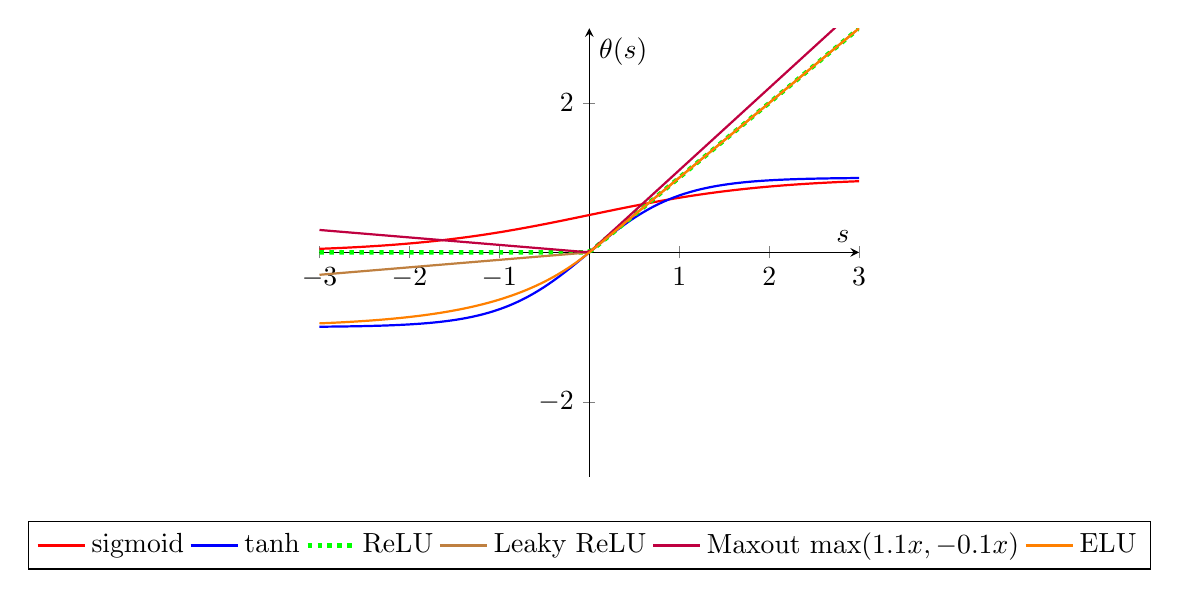
\begin{tikzpicture}
    \begin{axis}[
    axis lines=middle,
    xmin=-3, xmax=3,
    ymin=-3, ymax=3,
    xlabel={$s$},
    ylabel={$\theta(s)$},
    legend style={at={(0.5,-0.1)},anchor=north,legend columns=-1},
    cycle list name=color list
]

    % Sigmoid function
    \addplot[domain=-3:3, samples=100, red, thick] {1/(1 + exp(-x))};
    \addlegendentry{sigmoid}

    % Tanh function
    \addplot[domain=-3:3, samples=100, blue, thick] {tanh(x)};
    \addlegendentry{tanh}

    % ReLU function
    \addplot[domain=-3:3, samples=100, green, ultra thick, dotted] {max(0, x)};
    \addlegendentry{ReLU}
    % Leaky ReLU function
    \addplot[domain=-3:3, samples=100, brown, thick] {(x < 0) * 0.1 * x + (x >= 0) * x};
    \addlegendentry{Leaky ReLU}

    % Maxout function (example with alpha_1=1, beta_1=1, alpha_2=-1, beta_2=0)
    \addplot[domain=-3:3, samples=100, purple, thick] {max(1.1*x, -0.1*x)};
    \addlegendentry{Maxout $\max(1.1x, -0.1x)$}

    % ELU function
    \addplot[domain=-3:3, samples=100, orange, thick] {(x < 0) * (exp(x) - 1) + (x >= 0) * x};
    \addlegendentry{ELU}

    \end{axis}
    \end{tikzpicture}
    \caption{Common Activation Functions}
    \label{fig:actv-funcs}
\end{figure}

% \[
% \theta(s) = \tanh(s) = \frac{e^s - e^{-s}}{e^s + e^{-s}}
% \]

% \begin{figure}[H]
%     \centering
% \begin{tikzpicture}
% \begin{axis}[
%     axis lines=middle,
%     xmin=-3, xmax=3,
%     ymin=-1.5, ymax=1.5,
%     xlabel={$s$},
%     ylabel={$\theta(s)$},
%     legend pos=north west
% ]

% % Linear function
% \addplot[domain=-3:3, samples=2, green, thick] {x};
% \addlegendentry{linear}

% % Tanh function
% \addplot[domain=-3:3, samples=100, blue, thick] {tanh(x)};
% \addlegendentry{tanh}

% % Hard threshold (step) function
% \addplot[domain=-3:0, samples=2, red, thick] {-1};
% \addplot[domain=0:3, samples=2, red, thick] {1};
% \addlegendentry{hard threshold}

% \end{axis}
% \end{tikzpicture}
%     \caption{Activation Functions}
%     \label{fig:actv-funcs}
% \end{figure}


\subsection{Backward Computation}
\begin{figure}[H]
    \centering
    \includegraphics[width=1\linewidth]{img/nnbc.png}
    
    
\end{figure}
\subsection{Backpropagation Algorithm}\label{BackPropAlgo}
Backpropagation is a cornerstone algorithm for training neural networks. It efficiently computes the gradient of the loss function with respect to the weights of the network.


\begin{definitionbox}{Backpropagation Algorithm Steps}
\begin{enumerate}
    \item Initialize all network weights \( w_{ij}^{(l)} \) randomly to break symmetry.
    \item For each iteration \( t = 1, 2, \ldots \) until convergence:
    \begin{enumerate}
        \item Select a data point \( (x_k, y_k) \) randomly or sequentially.
        \item \textbf{Forward Pass}:
        \begin{itemize}
            \item Compute the activation \( x_j^{(l)} \) of each layer \( l \) starting from the input layer and progressing through to the output layer.
        \end{itemize}
        \item \textbf{Backward Pass}:
        \begin{itemize}
            \item Compute the gradient of the loss function with respect to the activations \( \delta_j^{(l)} \), starting from the output layer and propagating back to the input layer.
        \end{itemize}
        \item \textbf{Update Weights}:
        \begin{itemize}
            \item Adjust the weights \( w_{ij}^{(l)} \) in the direction that most reduces the loss, typically using a learning rate \( \eta \) and the gradient \( \delta_j^{(l)} \).
            \item The update can be done using a single data point (Stochastic Gradient Descent), a minibatch of data points, or the entire dataset (batch gradient descent).
        \end{itemize}
    \end{enumerate}
    \item After sufficient iterations or upon convergence, return the final weights \( w_{ij}^{(l)} \).
\end{enumerate}
\end{definitionbox}

\subsection*{Regularisation Techniques}
Regularisation is employed to prevent overfitting and improve generalisation. Common techniques include:
\begin{itemize}
    \item \( L2 \) regularisation (weight decay): Adds a penalty term to the loss function proportional to the sum of the squares of the weights.
    \item \( L1 \) regularisation: Adds a penalty proportional to the sum of the absolute values of the weights.
    \item Dropout: During training, randomly sets a subset of weights to zero to prevent co-adaptation of neurons.
\end{itemize}

\begin{examplebox}{Example Neural Networks Question}
\begin{figure}[H]
    \centering
    \includegraphics[width=0.5\linewidth]{img/nn_eg_q.png}
\end{figure}

\subsubsection*{Question}
Given this neural network, propose a non-linearity activation function, draw this function and its gradient in a figure.

\subsubsection*{Solution:}
% \begin{figure}[H]
%     \centering
%     \includegraphics[width=0.5\linewidth]{img/eg_sol_nn.png}
    
    
% \end{figure}


\begin{figure}[H]
    \centering
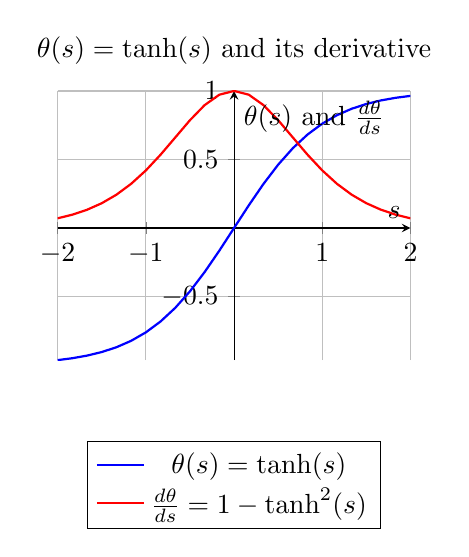
\begin{tikzpicture}
\begin{axis}[
    title={$\theta(s) = \tanh(s)$ and its derivative},
    axis lines=middle,
    width=0.5\textwidth,
    height=5cm,
    grid=major,
    domain=-2:2,
    legend style={at={(0.5,-0.3)},anchor=north },
    xlabel={$s$},
    ylabel={$\theta(s)$ and $\frac{d\theta}{ds}$},
]
% tanh function
\addplot[blue, thick] {tanh(x)};
\addlegendentry{$\theta(s) = \tanh(s)$}

% derivative of tanh function
\addplot[red, thick] {1 - (tanh(x))^2};
\addlegendentry{$\frac{d\theta}{ds} = 1 - \tanh^2(s)$}
\end{axis}
\end{tikzpicture}
\\

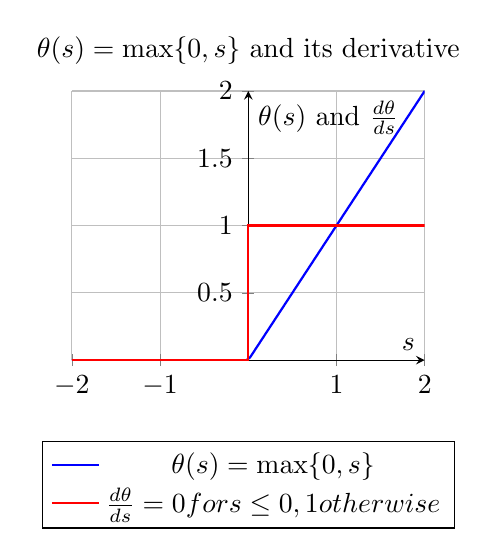
\begin{tikzpicture}
\begin{axis}[
    title={$\theta(s) = \max\{0, s\}$ and its derivative},
    axis lines=middle,
    width=0.5\textwidth,
    height=5cm,
    grid=major,
    domain=-2:2,
    legend style={at={(0.5,-0.3)},anchor=north },
    xlabel={$s$},
    ylabel={$\theta(s)$ and $\frac{d\theta}{ds}$},
    samples=100,
]
% ReLU function
\addplot[blue, thick] {max(0,x)};
\addlegendentry{$\theta(s) = \max\{0, s\}$}

% derivative of ReLU function
\addplot[red, thick, const plot mark mid] {x > 0 ? 1 : 0};
\addlegendentry{$\frac{d\theta}{ds} = 0 \text{ for } s \leq 0, 1 \text{ otherwise}$}

\end{axis}
\end{tikzpicture}
\end{figure}


\subsubsection*{Question}
Discuss what happens if we use \( x \) as input, \( \theta(s) = s \) as the activation function and \( W_l \) as a matrix of weights in layer \( l \). Can \( \theta(s) = s \) be achieved with \( \text{tanh}(s) \)?

\subsubsection*{Solution:} 
If the activation function is the identity function \( \theta(s) = s \), then the output of each layer in the neural network is a linear transformation of the input. The network effectively becomes a single linear model, as all weights between layers can be directly multiplied, like a product of matrices $\mathbf{w}_{L}^{\top}W_{L-1}W_{L-2}\ldots W_{1}\mathbf{x}=\mathbf{w}_{*}^{\top}\mathbf{x}$. This is because because the composition of linear functions is itself a linear function.\\

This means that the overall network can only represent linear relationships between the input and output.\\

\( \text{tanh}(s) \) is a non-linear function, and their general use is what allows neural networks to capture non-linearities and complex patterns in the data.\\

Therefore in general, \( \theta(s) = s \) cannot be achieved with \( \text{tanh}(s) \) because \( \text{tanh}(s) \) is non-linear. However, \(\text{tanh}(s) \) does approximate the linear function partially, so using regularisation, we can shrink the weights and biases so the output of \( \text{tanh}(s) \) is approximately linear for the range of inputs the network receives, then \( \text{tanh}(s) \) could approximate \( \theta(s) = s \).

\begin{figure}[H]
\centering
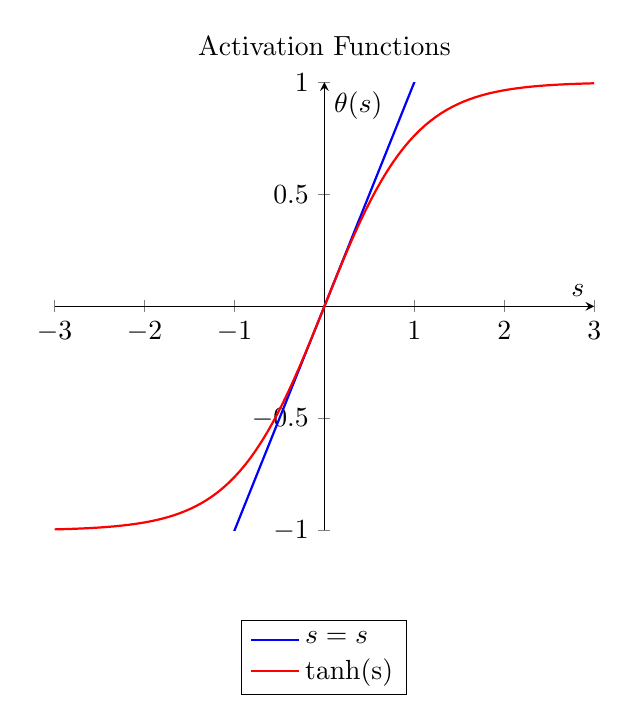
\begin{tikzpicture}
\begin{axis}[
    axis lines=middle,
    xmin=-3, xmax=3,
    ymin=-1, ymax=1,
    xlabel={$s$},
    ylabel={$\theta(s)$},
    legend style={at={(0.5,-0.2)},anchor=north},
    legend cell align={left},
    cycle list name=color list,
    title={Activation Functions}
]
% Linear function
\addplot[domain=-3:3, samples=100, blue, thick] {x};
\addlegendentry{$s=s$}

% Tanh function
\addplot[domain=-3:3, samples=100, red, thick] {tanh(x)};
\addlegendentry{tanh(s)}

\end{axis}
\end{tikzpicture}
\caption{Linear and Hyperbolic Tangent Activation Functions}
\end{figure}


\subsubsection*{Question}
Given input vector \( \mathbf{x} = (4, -8, 4) \) use the proposed non-linearity from question i) to calculate outputs of all neurons and \( h(\mathbf{x}) \).

\subsubsection*{Solution:}
The outputs \( x_j^{(l)} \) are calculated by applying the activation function \( \theta(s) \) to the weighted sum of the inputs:
\[ x_j^{(l)} = \theta\left( \sum_{i=0}^{d^{(l-1)}} w_{ij}^{(l)} x_i^{(l-1)} \right). \]
Using the ReLU activation function \( \theta(s) = \max(0, s) \), we get:
\begin{align*}
f_a &= \max(0, 1 + 0.25 \cdot 4 + 0.75 \cdot (-8) + 0.75 \cdot 4) = 0, \\
f_b &= \max(0, 1 + 0.5 \cdot 4 + 0.125 \cdot (-8) + 0.25 \cdot 4) = 3, \\
h(\mathbf{x}) &= f_c = \max(0, 0.5 + 0.5 \cdot 0 + 0.125 \cdot 3) = 0.875.
\end{align*}



\subsubsection*{Question}
Given the learning rate \( \eta = 0.1 \), ReLU activation, and a training example \( x = (4, -8, 4) \) with its label \( y = 2 \), we want to apply the backpropagation algorithm to update the weight \( w_{3,b}^{(2)} \) using the \( L_2 \) loss function without regularisation.

\subsection*{Solution:}
Using the outputs from forward propagation, the \( L_2 \) loss function \( \ell_2(f_c, y) \) is given by:
\[ \ell_2(f_c, y) = \frac{1}{2}(f_c - y)^2 = \frac{1}{2}(0.875 - 2)^2 = 0.63. \]

Since we are using ReLU activation, the derivative of the activation function \( \theta'(s) \) with respect to the pre-activation \( s \) is:
\[ \theta'(s) = \frac{\partial}{\partial c} \max(0, c) = 
\begin{cases} 
1 & \text{if } c > 0 \\
0 & \text{otherwise}
\end{cases}.
\]

The gradient of the loss with respect to the output of neuron \( c \) is:
\[ \frac{\partial \ell}{\partial f_c} = (f_c - y) = (0.875 - 2) = -1.125. \]

The error term \( \delta_c \) for neuron \( c \) is the same as the gradient since the derivative of ReLU for positive inputs is 1:
\[ \delta_c = \frac{\partial \ell}{\partial f_c} \frac{\partial f_c}{\partial c} =\frac{\partial \ell}{\partial f_c}  \frac{\partial  \max(0, c) }{\partial c}= -1.125. \]

The gradient of the loss with respect to the weight \( w_{3,b}^{(2)} \) is:
\[ \delta_b = \delta_c \frac{\partial c}{\partial w_{3,b}^{(2)}} = -1.125 \cdot 0.125 = -0.14. \]

The weight update rule for \( w_{3,b}^{(2)} \) is:
\[ w_{3,b}^{(2)} \leftarrow w_{3,b}^{(2)} - \eta x_3 \delta_b. \]

Substituting the values, we get:
\[ w_{3,b}^{(2)} \leftarrow w_{3,b}^{(2)} + 0.1 \cdot 4 \cdot 0.14. \]

\subsubsection*{Question}
Write down the main steps of the backpropagation algorithm.

\subsubsection*{Solution:} See \ref{BackPropAlgo}

\subsubsection*{Question}
What is the role of the learning rate in gradient descent and what are the risks of setting the learning rate too large or too small?

\subsubsection*{Solution:}
The learning rate \( \eta \) affects the speed of convergence. A small \( \eta \) may result in a very long optimisation process, whereas a large \( \eta \) can lead to oscillations near the function's minimum or cause divergence.

\end{examplebox}
\subsection{Remarks on Neural Networks}

\begin{itemize}
    \item Any kind of features can be learned, Neural Networks are called universal approximators as a result. Also, adding extra hidden layers may exponentially reduce the number of nodes needed.
    \item They are hard to interpret, and may not generalise well as their VC-dimensions are usually high.
    \item They achieve state-of-the-art performance in many areas, in different forms, such as Convolutional Neural Networks (CNN) for image processing and Recurrent Neural Networks (RNN) for speech and natural language processing.
    \item They work well with a lot of data, and can be used with various regularisers and target functions.
\end{itemize}

% All the weights $\mathbf{w} = \{w_{ij}^{(l)}\}$ determine $h(\mathbf{x})$

% Error on example $(\mathbf{x}_n, y_n)$ is

% \[ e(h(\mathbf{x}_n), y_n) = e(\mathbf{w}) \]

% To implement SGD, we need the gradient

% \[ \nabla e(\mathbf{w}): \frac{\partial e(\mathbf{w})}{\partial w_{ij}^{(l)}} \text{ for all } i, j, l \]
